\chapter{Introducción y objetivos}
\label{cap:capitulo_1}
\pagenumbering{arabic}

\begin{quote}
	\small \flushright ``\textit{Una partitura también es un lenguaje.}'' \\
	--- Profesor Buenaventura Clares Rodríguez (2013).
\end{quote}

\vspace{4em}

\section{Contexto}

Llegado el momento de cursar la asignatura ''Proyectos Informáticos'' de la titulación, iniciamos los preparativos para desarrollar un proyecto propuesto por el Departamento de Electrónica y Tecnología de Computadores de la Universidad de Granada.

Para plantearlo, nos hemos fijado en numerosas iglesias de Granada, que incorporan órganos de tubos, instrumentos muy complejos, muchos de ellos formando parte del inmobiliario, y merecedores de un gran reconocimiento por la artesanía y la calidad de su construcción. Lamentablemente, muchos de ellos están en un estado de abandono, debido principalmente a que si no se tocan regularmente, se deterioran y no se reparan, y al no hacerlo, no se pueden tocar, cayendo en un círculo vicioso.

Además, creemos interesante la idea de que se pueda hacer sonar un órgano aunque no haya organista, dando la posibilidad tanto de acompañar celebraciones litúrgicas como de tener música de fondo durante el horario de visitas.

\section{Objetivos}

Nuestro propósito es ingeniar un sistema capaz de \textbf{interpretar partituras musicales en un órgano} suplantando las pulsaciones del artista, lo que incluye los siguientes objetivos:

\begin{enumerate}
	\item Analizar la \textbf{mecánica real} de un órgano.
	
	\begin{enumerate}
		\item Tomar \textbf{medidas completas} de cada uno de los teclados, los pedales y las palancas de registros.
		\item \textbf{Diseñar en 3D} los componentes principales del instrumento.
		\item Determinar la \textbf{presión} necesaria para mover cada tecla, cada pedal y cada palanca del órgano.
	\end{enumerate}
	
	\item Estudiar la comunicación entre el \textit{software} y el \textit{hardware}, incluyendo todos los \textbf{componentes electrónicos} que habrá de incluir.
	
	\item Plantear distintas \textbf{alternativas de sistemas empotrados} que sirvan de soporte de programación.
	
	\item Analizar el \textbf{protocolo \acrshort{MIDI}} como formato de archivo para almacenar partituras.
	
	\item \textbf{Diseñar} el sistema \textit{software} que cubrirá varias vías de comunicación entre el usuario y la mecánica, lo que comprende:
	
	\begin{enumerate}
		\item Un \textbf{servicio en segundo plano}, que atienda:
		
		\begin{enumerate}
			\item Reproducción de archivos \acrshort{MIDI}.
			\item Comunicación inter-proceso.
			\item Receptor de un mando a distancia.
			\item Menú de control sobre el \textit{hardware}, con un ''modo Ingeniería''.
		\end{enumerate}
		
		\item Una \textbf{aplicación \textit{web}} para controlar el sistema, con soporte para:
		
		\begin{enumerate}
			\item Reproducir partituras electrónicas.
			\item Instalar nuevas piezas y gestionar listas de reproducción.
			\item Configurar el mando a distancia.
		\end{enumerate}
		
		\item Una \textbf{base de datos} como soporte de almacenamiento persistente.
		\item Un \textbf{protocolo de comunicación} entre la aplicación y el servicio.
	\end{enumerate}
	
	\item \textbf{Implementar} el sistema diseñado, como:
	
	\begin{enumerate}
		\item Un demonio para Linux.
		\item Un servicio \textit{web} sobre Apache y \acrshort{PHP}.
		\item Una base de datos MySQL.
	\end{enumerate}
	
	\item \textbf{Validar} junto al \textit{hardware} el proyecto desarrollado.
\end{enumerate}

Este proyecto atenderá al objetivo global pero \textbf{el desarrollo se centrará en la parte \textit{software}}, ya que el \textit{hardware} requiere competencias de Ingeniería Electrónica e Industrial, y será objeto del proyecto de D. Mikel Aguayo Fernández.

Para abordarlo, hemos contado con la colaboración de \textbf{Juan Rodríguez Ruiz}, responsable del órgano de la \textbf{Parroquia de la Encarnación de Santa Fe}, que nos ha dado acceso tanto al instrumento como a asombrosos datos sobre su historia y su construcción.

\smallskip

\begin{figure}[H]
\noindent \begin{centering}
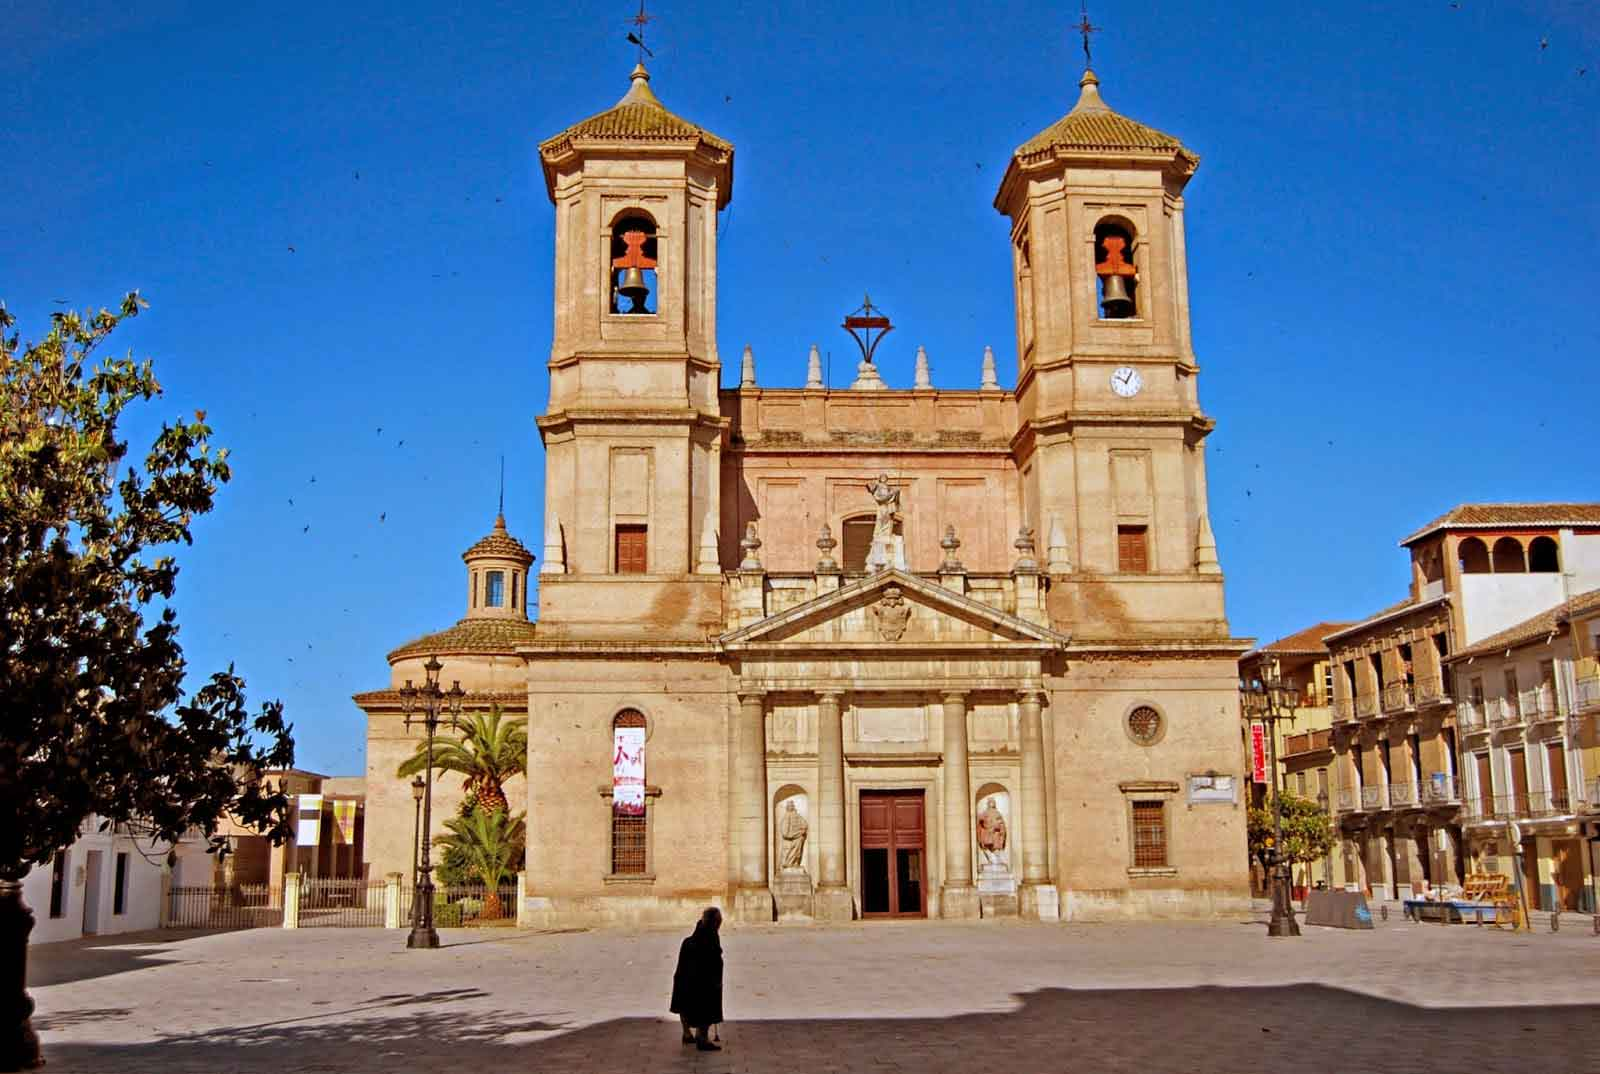
\includegraphics[width=\linewidth]{capitulo1/parroquia}
\par\end{centering}
\smallskip
\caption[Parroquia de la Encarnación de Santa Fe.]{\label{fig:parroquia} Parroquia de la Encarnación de Santa Fe. \cite{iglesias_granada}}
\end{figure}

\newpage

\section{Contenido y estructura capitular}

Una vez planteado el problema, utilizaremos el \textbf{modelo de desarrollo en cascada} para continuar el resto del proyecto.

El modelo en cascada ordena rigurosamente las etapas del proceso, de forma que cada tarea se inicia cuando su precedente finaliza, tal como se expone en la siguiente ilustración:

\smallskip

\begin{figure}[H]
	\noindent \begin{centering}
		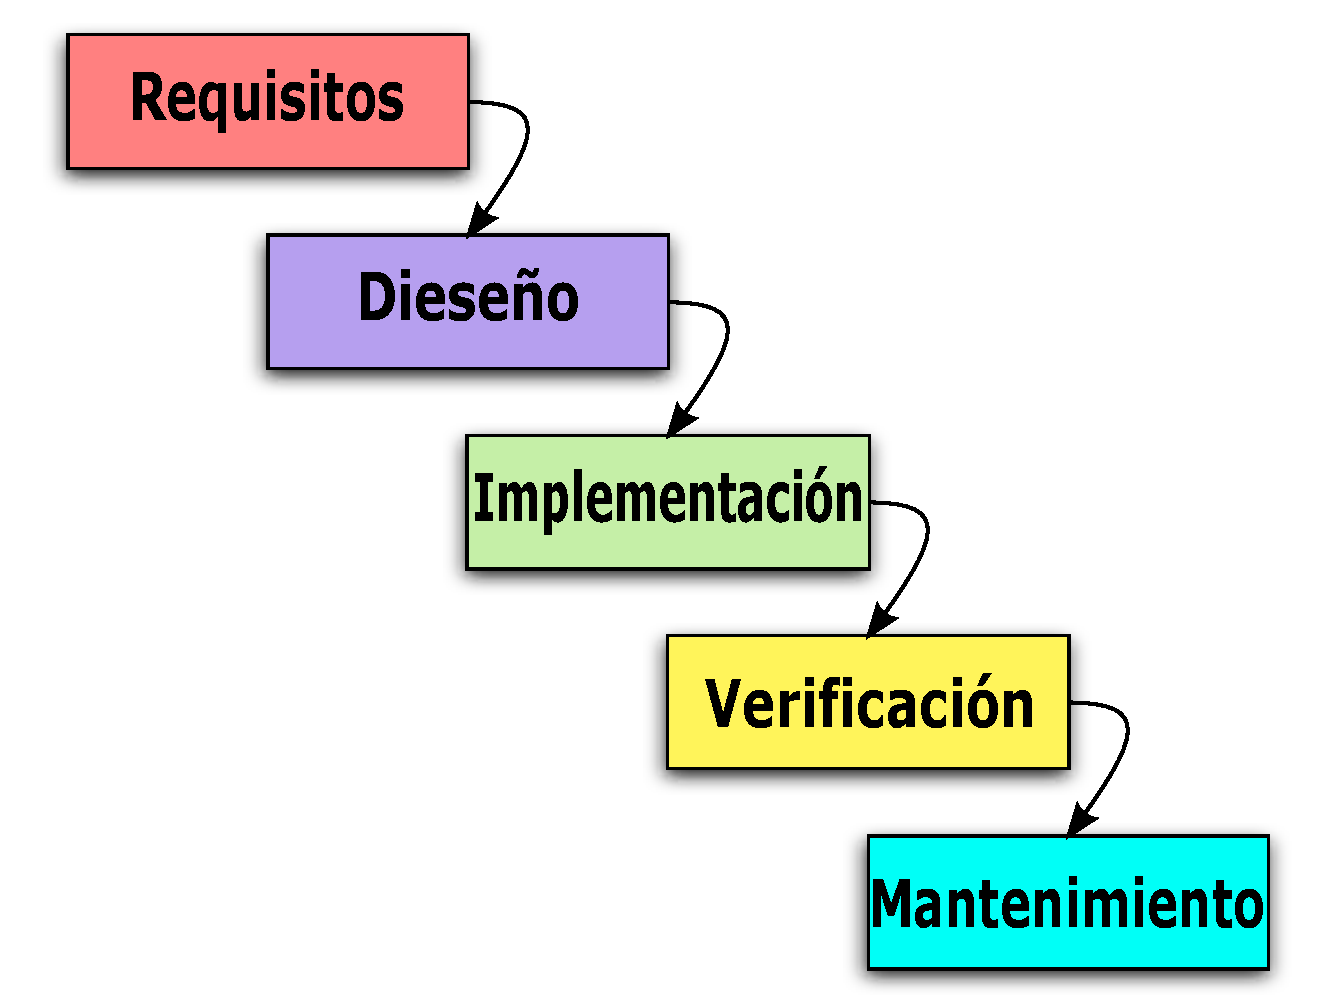
\includegraphics[width=\linewidth/2]{capitulo1/cascada}
		\par\end{centering}
	\smallskip
	\caption[Modelo de desarrollo en cascada.]{\label{fig:cascada} Modelo de desarrollo en cascada. \cite{wiki_cascada}}
\end{figure} 

\smallskip

Basándonos en la figura anterior, definiremos el resto de capítulos de esta memoria.

\begin{itemize}

\item \textbf{Capítulo 2:} En este capítulo especificaremos los requisitos que supone el diseño del sistema para alcanzar nuestro objetivo, así como indicar las fases del proyecto.

\item \textbf{Capítulo 3:} Vamos a analizar todos los elementos con los que vamos a interactuar, desde el teclado del órgano hasta el computador sobre el que funcionará nuestro \textit{software}. 

\item \textbf{Capítulo 4:} Plantearemos el diseño de la solución, haciendo Ingeniería el \textit{software}, que cumpla de la mejor manera posible los requerimientos del capítulo \ref{cap:capitulo_2}.

\item \textbf{Capítulo 5:} En esta parte explicaremos cómo hemos implementado la solución diseñada, y cómo hemos enfrentado los principales problemas que han surgido.

\item \textbf{Capítulo 6:} Vamos a validar el sistema poniéndolo en funcionamiento y probando que cumple los requisitos propuestos.

\item \textbf{Capítulo 7:} Expondremos la conclusión y las posibilidades que nos brinda el proyecto de cara al futuro.
  
\end{itemize}

\newpage
\clearpage{\pagestyle{empty}\cleardoublepage}
